
In this section, the dataset is first described, followed by the methodology. This is followed by some results and a discussion of those results. 
\subsection{Dataset}
We used the \emph{Wiki} test set first developed by the authors of GLOW \cite{roth}. They made the dataset available on their companion project website\footnote{\url{http://cogcomp.cs.illinois.edu/data}}. The Wiki data came with training data and test data and were extracted from `difficult'\footnote{As described by the GLOW authors.} Wikipedia paragraphs (baseline features in GLOW yield at least a 10 percent error rate on these extracted paragraphs). The training data was much larger than the test data. In their work, they first trained a sophisticated system using the training data and then evaluated both a ranker and linker on the test data. Since we're only evaluating unsupervised linking, we used only the test data. Note that the data consists of 40 documents with a total of 839 mentions (extracted by Stanford NER) in those documents. Some of these were nulls (that is, had no corresponding Wikipedia page according to the provided ground truth) and for others, the Wikipedia API returned multiple candidates (and which were hence ignored). In total, there were 724 mentions for which the API returned a single link. Some of these links were `wrong' in that they corresponded to a null in the ground truth or a \emph{different} Wikipedia page than what the API returned. On average, we found about 78 percent of the returned links to be correct. Thus, a naive approach that would randomly sample N links (we do use this as one of our baselines, in fact) would return between 75 and 78 percent on average.   
\subsection{Methodology}
We experimented with each of the features as well as their combinations, using three models: bag of words, bi-grams and tri-grams. For each model, two sets of experiments were conducted. Both experiments use $N$ as the independent variable, and for each document, mark the top N scoring (where the score is the dot product of the feature vectors) candidate links as correct. Accuracy is measured (that is, how many of these chosen links are correct) against N. For example, if all N chosen links are correct, the accuracy is 100 percent. Although N does not technically represent \emph{recall}, it is somewhat analogous, since the higher N is, the more links will show up in a document. Note however that since we have multiple documents, there are two different ways (at least) to calculate accuracy for a given value of N when the algorithm is run on all documents. The first, which we call the \emph{surface forms accuracy}, is to compute the accuracy of disambiguation across the full set of mentions in the entire corpus. There is no averaging across documents. The second is to compute the accuracy for each document individually, and to then average accuracies across documents, with each document getting equal weight (\emph{documents accuracy}). As a simple example of the difference, suppose there are two documents with 20 mentions in the first document and 40 mentions in the second. Suppose, on average, that the accuracy on the first document is 80 percent, and on the second is 75 percent. The documents accuracy would then simply be 77.5 percent. However, the surface forms accuracy would be $(.75*40+.80*20)/60=76.667$ percent. We show the results for both forms of averaging in the experiments. Recall that one of the features proposed is that of stop words removal. Stopwords were taken from a Web resource\footnote{\url{http://ir.dcs.gla.ac.uk/resources/linguistic_utils/stop_words}}. We used two baselines: random selection of N candidates and normalized TF. By supplementing normalized TF with IDF, stop words removal or both, we measure the enhancement in performance for all the models.
\subsection{Results and Discussion}
The first interesting trend observed in all the figures is that we don't see a standard precision-recall curve where precision, or accuracy, goes down as N increases. What happens instead is that the figures yield a flat curve of about 78 percent for the surface forms accuracy and 77 percent for the documents accuracy. In general, absolute differences aside, the surface forms accuracy and documents accuracy curves were found to mirror each other closely (with only about one percent difference in absolute numbers) so we refer to a single curve in the following discussion (surface forms). The value of N at which accuracy seems to peak is between 15 and 20 for all the figures. \\
A somewhat surprising aspect is that the TF baseline actually performs worse than the random baseline till this peak value, after which it usually shows slight improvement before leveling off, along with the rest of the curves. Notice also that the combination of features (TF,IDF and stopwords) works best but except on the bigrams model the other features actually show better performance on lower values of N. The best performance for N between 2 and 5 was demonstrated by TF IDF on the trigrams model. Over that range, it briefly outperforms the combined three features of TF, IDF and stopwords.\\
It is interesting to compare the unsupervised performance with the supervised performance using a much more sophisticated method and features than what we've used (in the original GLOW paper) \cite{roth}. Using a trained linker, the authors were able to achieve about a 92 percent accuracy . However, as mentioned before, the training data was much larger than the test data and the ranker accuracy was assumed to be perfect. Thus, the only task addressed was determining the `nulls' in the ground truth. On the other hand, we had to rely on the Wikipedia API for our `ranker candidate'. Some of these were wrong. In this sense, the unsupervised linker problem is harder since we have to determine both nulls (mentions that don't correspond to a Wikipedia page at all in the gold standard) as well as mentions for which wrong links were returned by the API. Although the 10 percent difference is still considerable, we believe it can be narrowed by even better features.  An encouraging sign is that by using a tri-gram model with some intuitive enhancements we were experimentally able to push the accuracy to over 83 percent for a small practical range of N. 

\begin{figure}
\centering
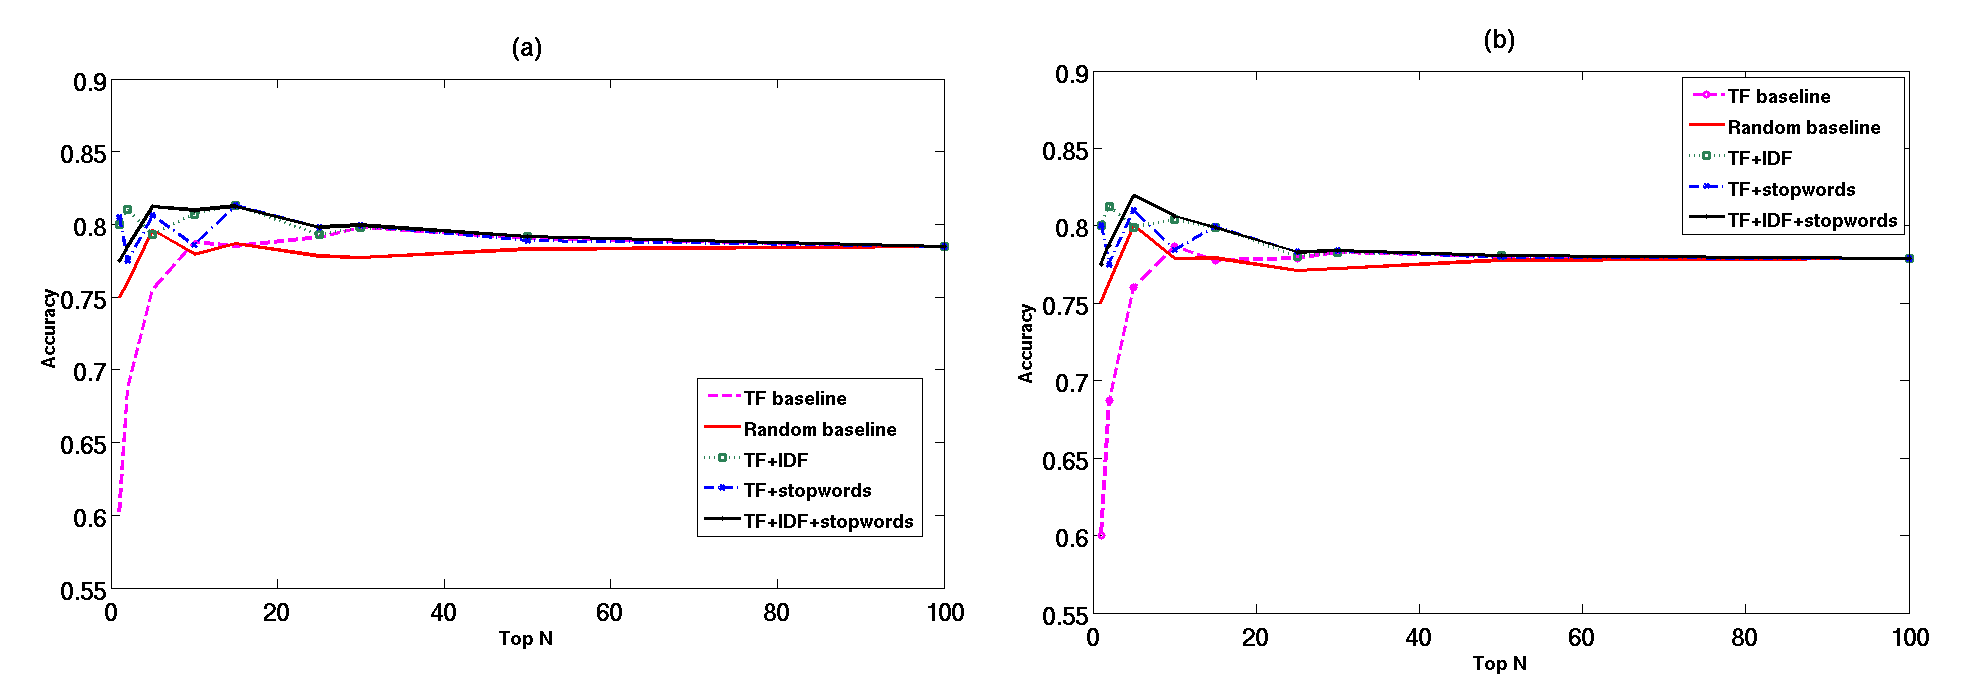
\includegraphics[height=5cm, width=12.5cm]{normal}
\caption{Results of the procedure when no n-gram features are employed. (a) represents surface forms accuracy and (b) shows documents accuracy}
\label{fig1}
\end{figure}
\begin{figure}
\centering
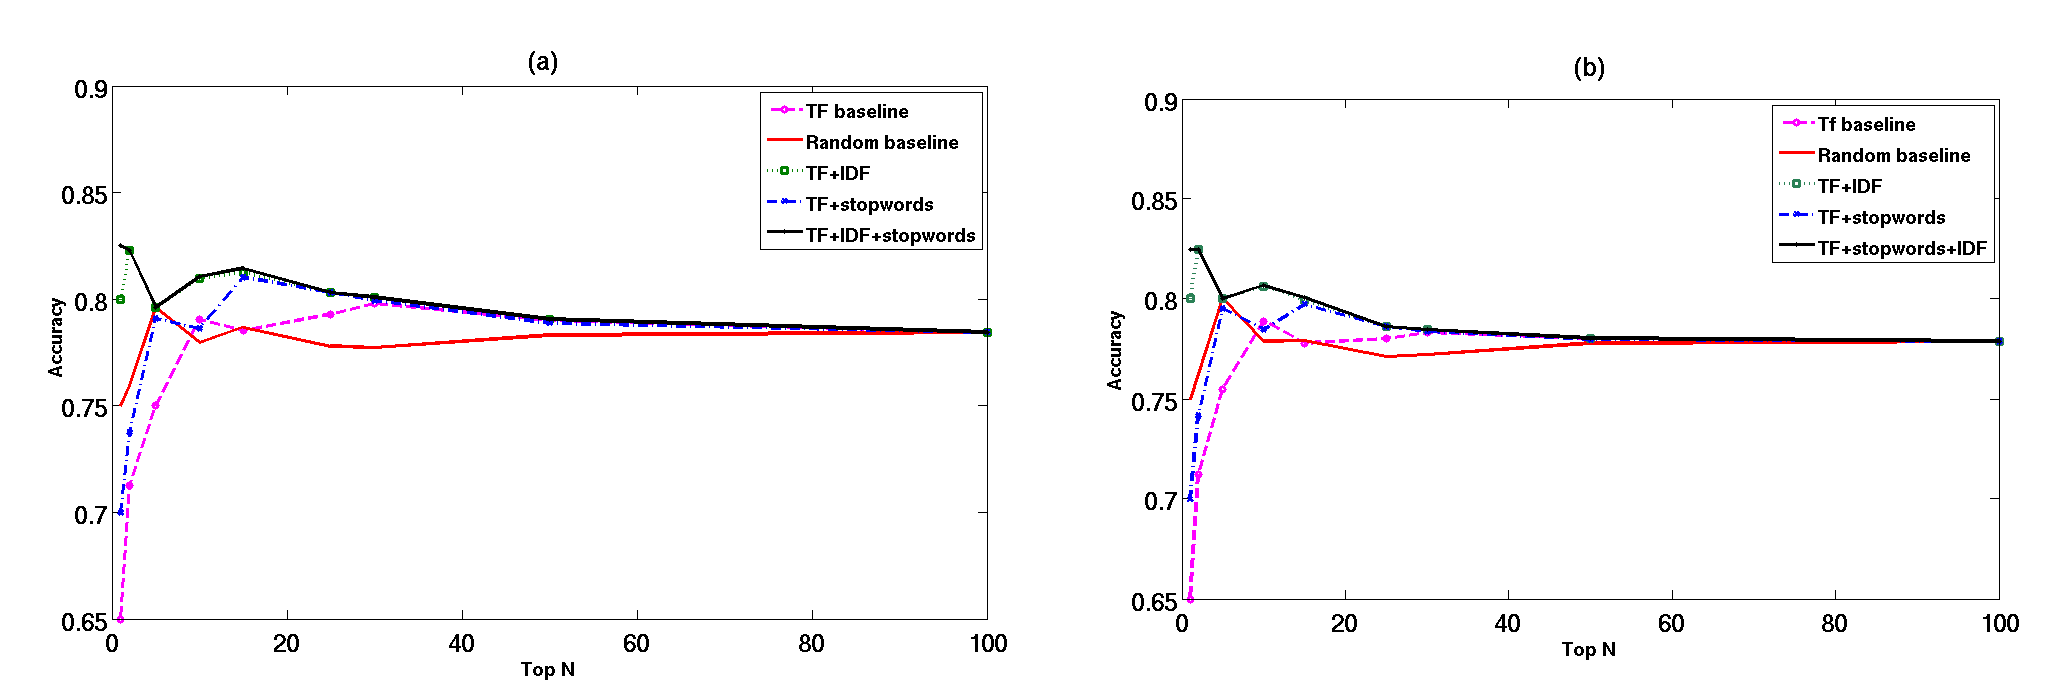
\includegraphics[height=5cm, width=12.5cm]{bigrams}
\caption{Results of the procedure when TF includes bi-gram features. (a) represents surface forms accuracy and (b) shows documents accuracy}
\label{fig1}
\end{figure}
\begin{figure}
\centering
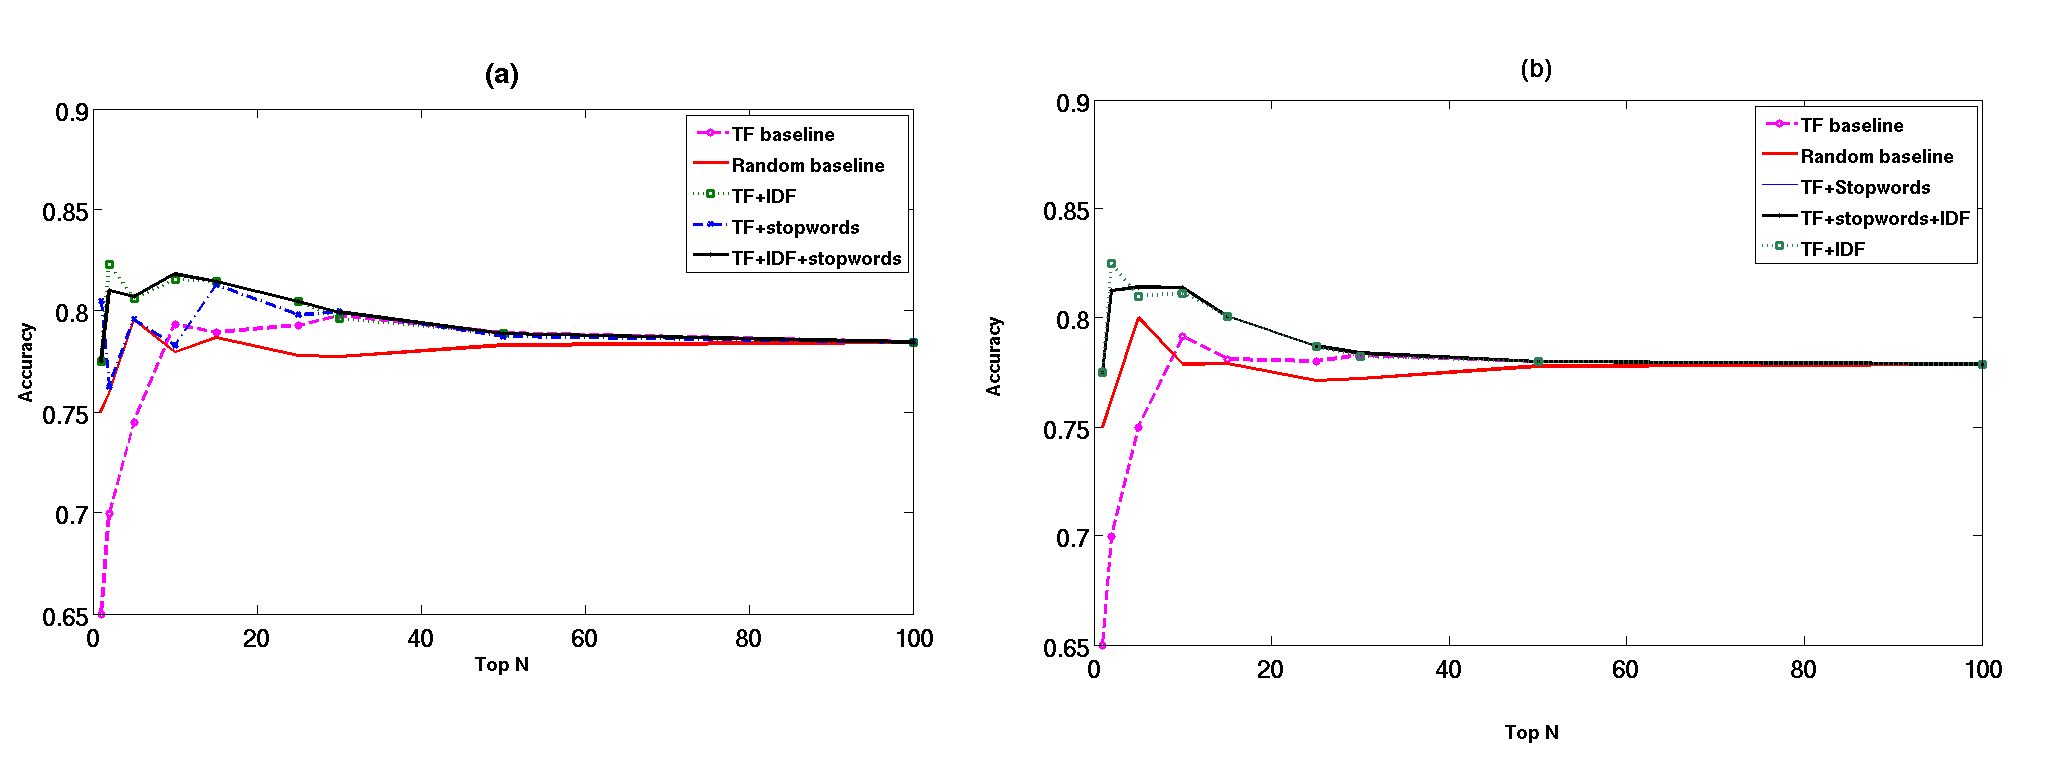
\includegraphics[height=5cm, width=12.5cm]{trigrams}
\caption{Results of the procedure when TF includes tri-gram features. (a) represents surface forms accuracy and (b) shows documents accuracy}
\label{fig1}
\end{figure}
